%このサンプルは過去の先輩が残してくれたものに,一部修正を加えたものです.


\documentclass[a4paper, twoside]{jarticle}
% a4paper : A4のサイズに設定
% twoside : 偶数/奇数ページで異なるレイアウト,bookのデフォルト.

\usepackage{tani_resume} % 卒論用
\usepackage{epstopdf}
\usepackage{graphicx}
\usepackage{ascmac} % レイアウトを綺麗にする
\usepackage{comment} % 複数行のコメントを使用できる

% 先輩方が全員記述しているため,記述した,検索しても用途が不明
% --- ここから ---
\alignbeforeskip -5mm
\alignafterskip -5mm
\eqnarraybeforeskip -5mm
\eqnarrayafterskip -5mm
\makeatletter
\newenvironment{figurehere}
  {\def\@captype{figure}}
  {}
\makeatother
% --- ここまで ---

\jptitle{千代田区空散歩アプリ「ちよダッシュ!」の開発} % タイトル
\etitle{} % 空白で構わない
\jpauthor{岩田匡裕・高山泰征・安田貴裕} % 名前
\eauthor{Masahiro Iwata, Taisei Takayama, Takahiro Yasuda} % 名前(ローマ字)
\course{谷聖一 研究室} % {谷聖一 研究室}で良い
\year{元} % 自分たちの代の年度
%多分これを見る頃には平成じゃなくなっているので誰かtani_reusme.styを変更する必要あり
% \rhead{\date{}}
% \date{\today}

\abstract{ % 概要
% 本演習では,iOS・Android に対応した千代田区散歩アプリ「ちよダッシュ!」のコンセプトとプロトタイプを基に,改良・改善を加えた正式版の開発とリリースを行なった.

% Google Map 上に古地図や文学テキストや言語資料を配置し,日本語日本文学の観点から近世・近代・現代を透かし見ることで江戸・東京圏を再 構築することを目指した Web アプリ「江戸・東京 WebGIS」をベースに,千代田区を興味を持って歩くことを目的として千代田区散歩アプリ「ちよダッシュ!」を開発した.本アプリは,iOS と Android に対応している.

本演習では,千代田区を楽しく歩くことで千代田区をより知ってもらうことを目的とした iOS と Android に対応した千代田区散歩アプリ「ちよダッシュ!」を開発した. このアプリはGoogle Map 上に古地図や文学テキストや言語資料を配置し, 日本語日本文学の観点から近世·近代·現代を透かし見ることで江戸·東京圏を再構築することを目指した Web アプリ「江戸·東京 WebGIS」を基礎にしている.
}

% 右上に最終更新時刻を表示する,バックアップを見返す際に便利
% 先輩方は完成時にはコメントアウトしている
% \compheading % 最終更新時刻

% \date{\now}


\begin{document} % 文書(開始)
\maketitle % タイトルを表示する
\begin{multicols}{2} % 2段落にする(開始)
\setcounter{page}{1} % ページ開始番号

% はじめに
\section{はじめに}

\subsection{人文学とデジタル・ヒューマニティーズ}
%%%人文科学とは%%%
人文学は,例えば,『「人間」とは何かということを様々な媒体や方法によって追求する,人間研究の基礎学』(\cite{huma})と言われている.\par
%%%デジタル%%%
近年,情報通信技術の発達などによりデジタル技術の発達がみられる.
%デジタル・ヒューマニティーズ
\cite{digihumu1}によると,「デジタル媒体による学術資料のアーカイブ構築,文化コンテンツの分析,学術成果の公開や展示の方法などを,文系・理系の枠組みを横断して研究するデジタル・ヒューマニティーズの動きが世界的に拡がっている」と言われている.\par

デジタル・ヒューマニティーズとは,\cite{digihumu2}によると,「人文学的問題を情報学的手法を用いて解くことにより新しい知識や視点を得ることや,人文学的問題を契機として新たな情報学の分野を切りひらくことなどを目指す,情報学と人文学の融合分野である」と言われている.

本演習では,地図上に配置した古今の名所旧跡の場所を巡る位置情報アプリを開発している.この活動は情報学と人文学を融合しているので,デジタル・ヒューマニティーズを体現してると言える.

% 「現代のWeb 地図上に古今の名所旧跡を図版・解説資料等とともに配置するアプリ」(\cite{tiyodagaku_houkokusyo})


\subsection{千代田学}
千代田区は,\cite{digi4}によると,11校の大学と「千代田区内大学と千代田区の連携協力に関する基本協定」を結んでいる.
その提携事業の一つとして,区内にある大学が千代田区の様々な事象を多様な切り口で調査・研究することを「千代田学」と名付け,その定着と発展を目指し,必要となる経費の一部を区が補助する「千代田学」提案制度を平成16年度より行っている.
% (\cite{digi5})<-意味不明

令和元年度「千代田学」提案制度に,日本大学からは「千代田ヴァーチャル時空散歩アプリちよダッシュ!の充実と展開」が採択されている.

\subsection{千代田区と日本大学}
千代田区は,1947年(昭和22年) 3月15日に麹町区と神田区が合併して誕生した.東京23区のほぼ中央に位置し,区の中央には皇居のある「千代田区千代田」があり,千代田区全体の約12\%が皇居の緑地となっている.また,1457年に築城された江戸城は「千代田城」とも呼ばれ,千代田区の名称の由来となっている(\cite{digi1}).\par
日本大学の前身である日本法律学校が誕生した地が千代田区(\cite{digi2})であり,現在では日本大学本部を始め,5つの学部が点在している.

\subsection{参加プロジェクト}
著者らが参加している千代田学プロジェクトというものは,千代田学の定着と発展,また各学校が区および地域と連携を図ることを目的とし,(\cite{chiyopro})「都心の魅力にあふれ,文化と伝統が息づくまち千代田」の実現という意義のもと活動が行われている.\par
日本大学では平成30年度に「WebGISを用いた千代田ヴァーチャル時空散歩アプリの構築」,令和元年度に「千代田ヴァーチャル時空散歩アプリ「ちよダッシュ!」の充実と展開」というプロジェクトで千代田学プロジェクトに参加している.


\section{先行研究}


\subsection{江戸・東京WebGISについて}
日本大学文理学部では平成22年度の文部科学省私立大学戦略的研究基盤形成支援事業(\cite{monka})において,東アジアにおける都市形成プロセスの統合的把握とそのデジタル化をめぐる研究のプロジェクトの研究の一環として,いくつかの研究成果を公開している.その一つとして「江戸・東京WebGIS」が公開されている.「江戸・東京WebGIS」は, Google Map 上に古地図や文学テキストならびに言語資料を配置し,日本語日本文学の観点から近世・近代・現代を透かし見ることで江戸・東京圏を再構築することを目指したWebアプリである.
% 現代の地図に近世期の地図「江戸切絵図」(1849-52年刊行)や近代期地図「東京市全図」(1907年刊行)を重ね合わせ,これら古地図の透過表示することができ,近世・近代・現代を透かし見ることができる.このような重層的地図に,近世・近代・日本語に関連する資料を配置している.(\cite{webgis_gaiyo})

\subsection{江戸・東京ものがたりについて}
「江戸・東京WebGIS」はスマートフォンでも閲覧することができていたが,データ量が多く動作が重いなどの問題があり不便であった.そのため,スマートフォンでの使用に特化したアプリ「江戸・東京ものがたり」が昨年度の卒業演習により作成された(\cite{houkokusyo_30}).このアプリは今年度の演習において利用規約などを追加した正式版を作成し,一般公開を目指しているため Google Play ストアと App Store で一般公開をするために現在審査中である.

\subsection{「ちよダッシュ!」の背景と目的}
平成30年度の「千代田学」調査・研究(\cite{tiyokenkyu})においてWebGISを用いた千代田ヴァーチャル時空散歩アプリの構築を研究テーマとし,「千代田ヴァーチャル時空散歩」ができるスマートフォンアプリとして,「ちよダッシュ!」のプロトタイプが作成された(\cite{tiyodagaku_houkokusyo}).

「ちよダッシュ!」は「江戸・東京WebGIS」をベースとした,地図上のピンの場所を巡る位置情報アプリである.散歩の友としてこのアプリを利用し誰でも楽しめることをコンセプトとしており,千代田区に足を運んでいただき千代田区に興味をもってもらうことを目的として,開発されたスマートフォン用のアプリである.

\subsection{昨年度の「ちよダッシュ!」}
「ちよダッシュ!」開発は昨年度から行われており,昨年度はコンセプト策定とプロトタイプアプリ製作,今年度は開発とリリースを行った.昨年度の演習において,コンセプトは「散歩の友としてこのアプリを利用し誰でも楽しめること」と決められた.また,プロトタイプには, Google Maps 上での資料閲覧機能とスタンプラリー機能が実装された.
% このように「ちよダッシュ!」は段階を分けて作成した.

\section{本演習}

\subsection{今年度の「ちよダッシュ!」}
今年度本演習で開発した「ちよダッシュ!」は昨年度のプロトタイプをベースに新たな機能を追加した.
その追加機能によりアプリをスマートフォンでさらに扱いやすく,ユーザに楽しんで利用してもらえることを目指した.

\subsection{スプラッシュ画面}
% デザインは外部に依頼して作成.
% 千代田区がシンボルにしている「松・桜・白鳥」と古地図を用いている.(図 1 参照)
デザインは著者らが考えたいくつかの案の中から,古地図を背景にして千代田区がシンボルにしている「松・桜・白鳥」を取り入れ,画面中央に「ちよダッシュ!」のロゴを入れる案を採用して,外部にイラスト作成を依頼した(図 1 参照).

\begin{figurehere}
\begin{center}
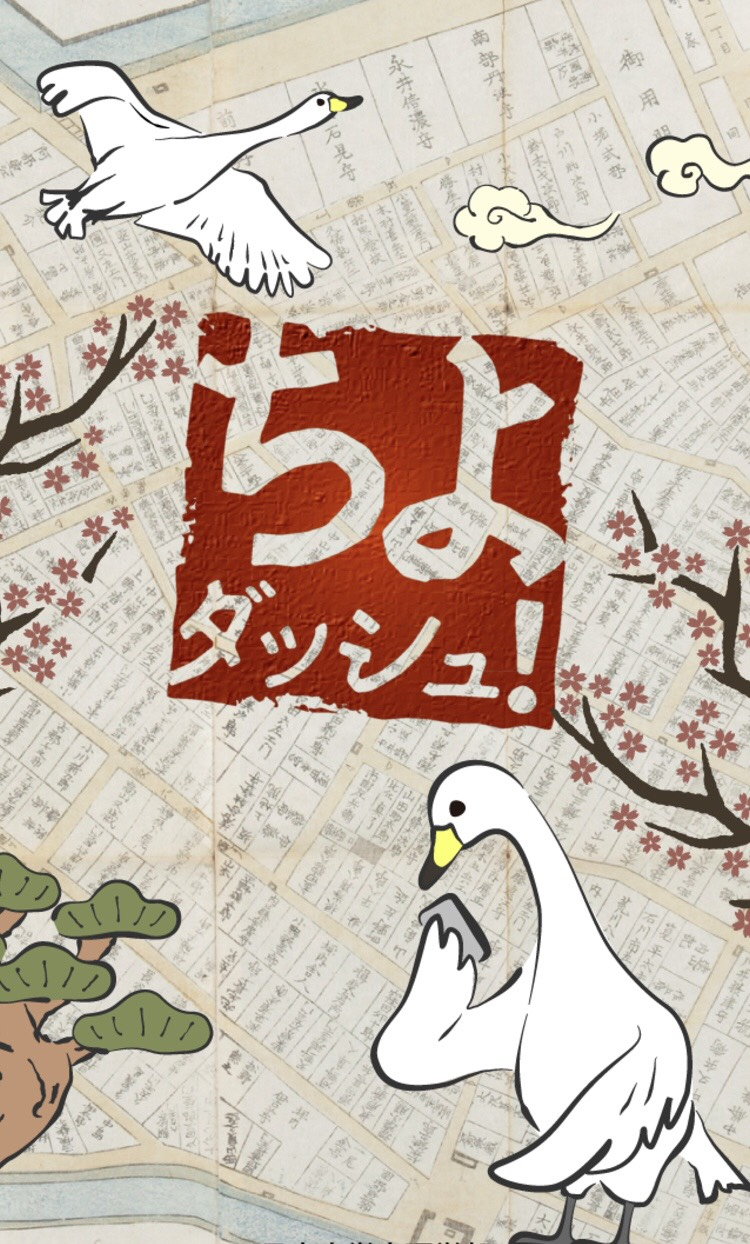
\includegraphics[bb=30 50 550 1300,width=3cm]{./image01.jpg}%%750*1334(100%)でスクショ[大きさ 横 縦,width]
\end{center}
\caption{スプラッシュ画面}\label{fig:1}
\end{figurehere}

\subsection{利用規約同意画面}
利用規約を上のボタンにより日本語版と英語版に切り替えをできるようにした.
また「今後表示しない」のチェックボックスにチェックを入れてアプリを始めると,次のアプリ起動時から利用規約画面が表示されなくなる機能を追加した(図 2,3 参照).
\begin{figurehere}
\begin{center}
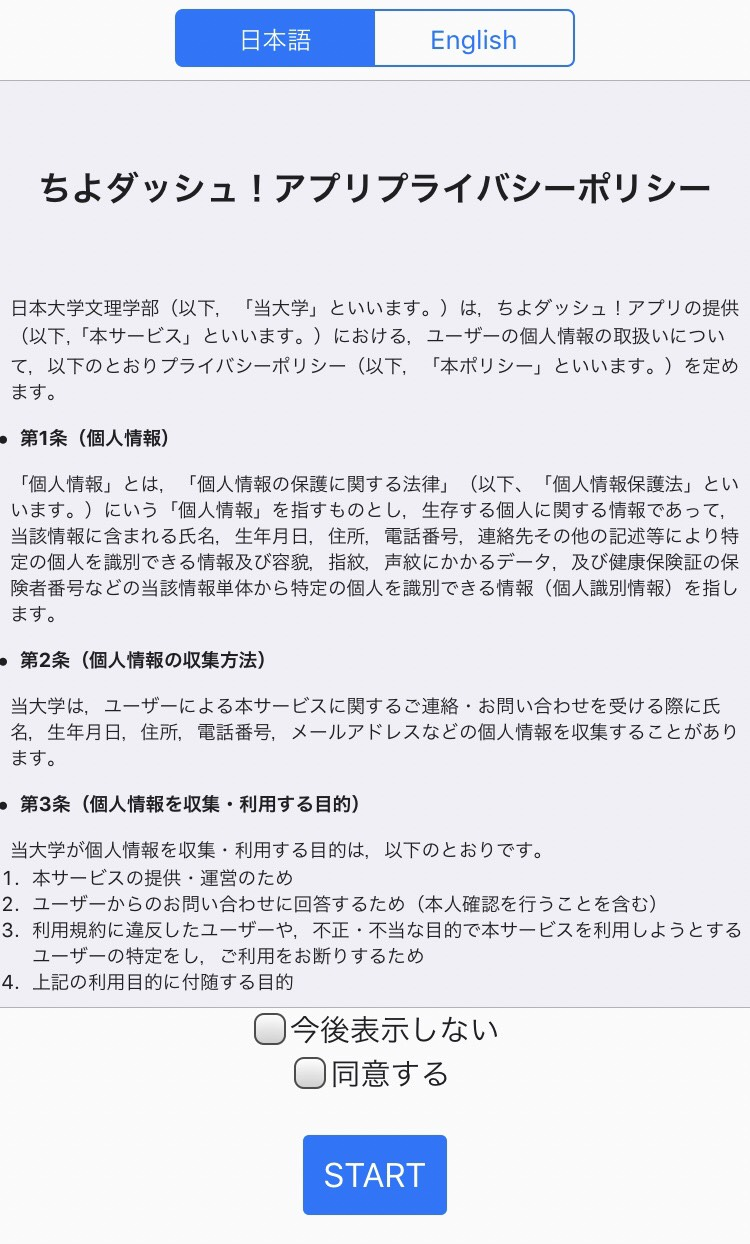
\includegraphics[bb=30 50 550 1300,width=3cm]{./image02.jpg}%%750*1334(100%)でスクショ[大きさ 横 縦,width]
\end{center}
\caption{利用規約画面 日本語版}\label{fig:2}

\begin{center}
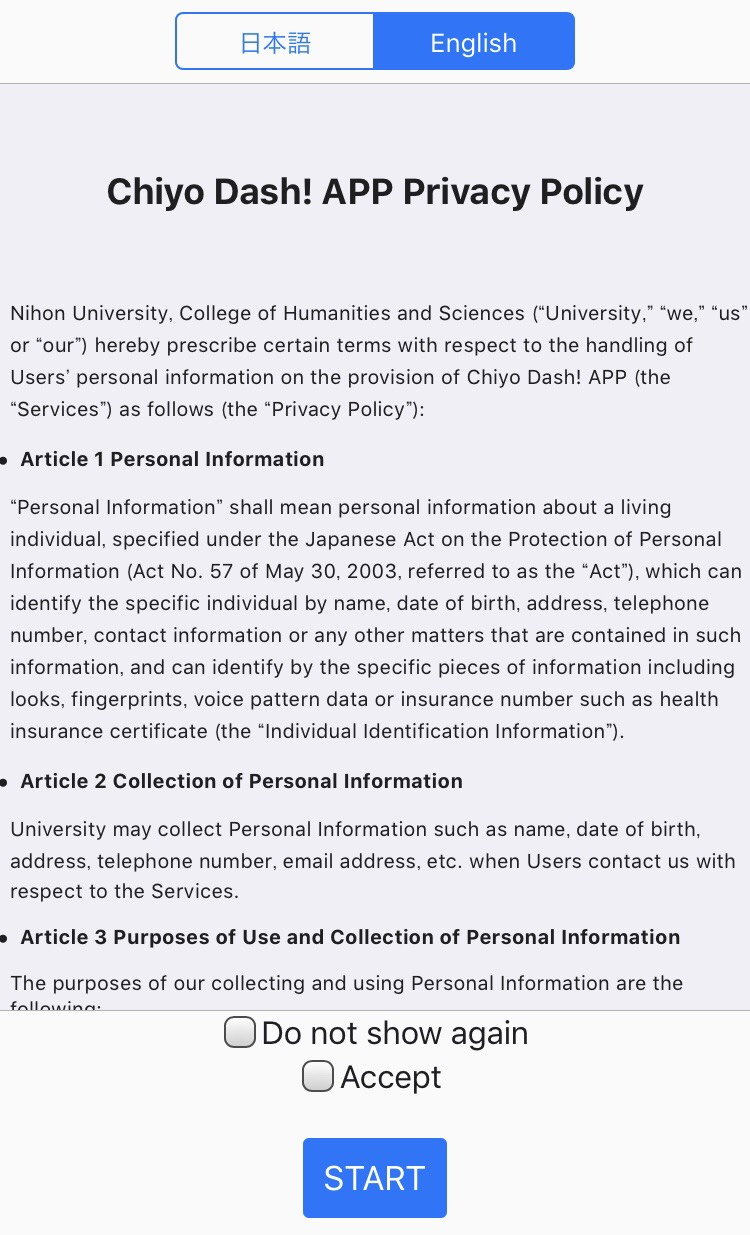
\includegraphics[bb=30 50 550 1300,width=3cm]{./image03.jpg}%%750*1334(100%)でスクショ[大きさ 横 縦,width]
\end{center}
\caption{利用規約画面 英語版}\label{fig:3}
\end{figurehere}
% また同意するにチェックを入れないとアラートが表示される.

% \begin{center}
% 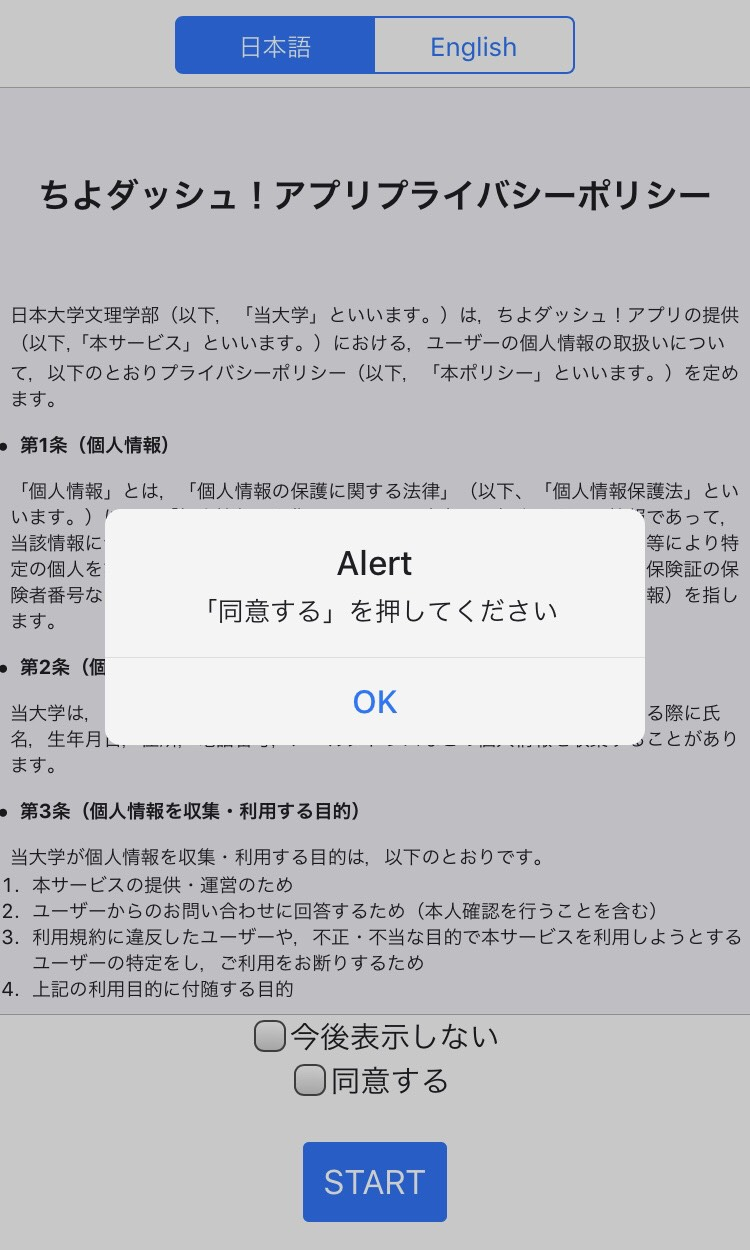
\includegraphics[bb=30 50 550 1300,width=3cm]{./image04.jpg}%%750*1334(100%)でスクショ[大きさ 横 縦,width]
% \end{center}
% \caption{利用規約画面3}\label{fig:4}
% \end{figurehere}

\subsection{スタンプ獲得の有無によるピン表示の変更}
スタンプを獲得すると,ピンの画像が黒点のあるものからないものに変化する機能を実装した(図 4,5 参照).
\begin{figurehere}
\begin{center}
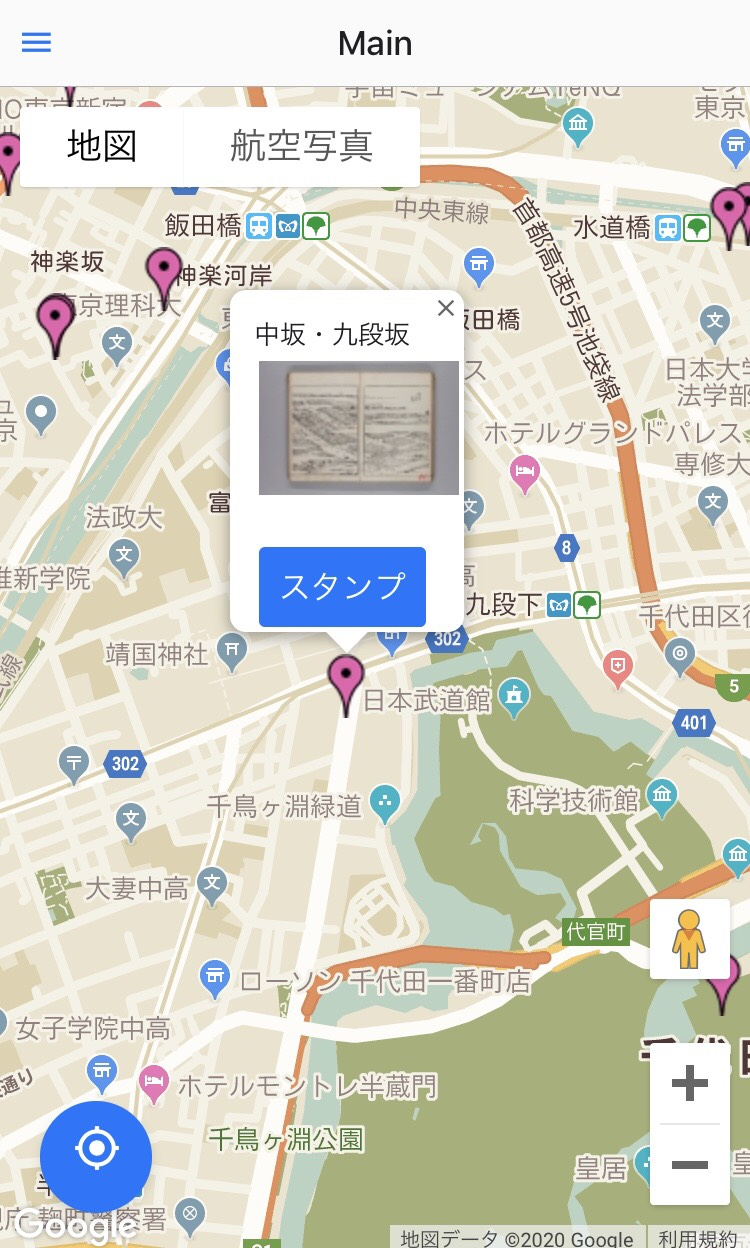
\includegraphics[bb=30 50 550 1300,width=3cm]{./image05.jpg}%%750*1334(100%)でスクショ[大きさ 横 縦,width]
\end{center}
\caption{スタンプ獲得前(黒点あり)}\label{fig:4}

\begin{center}
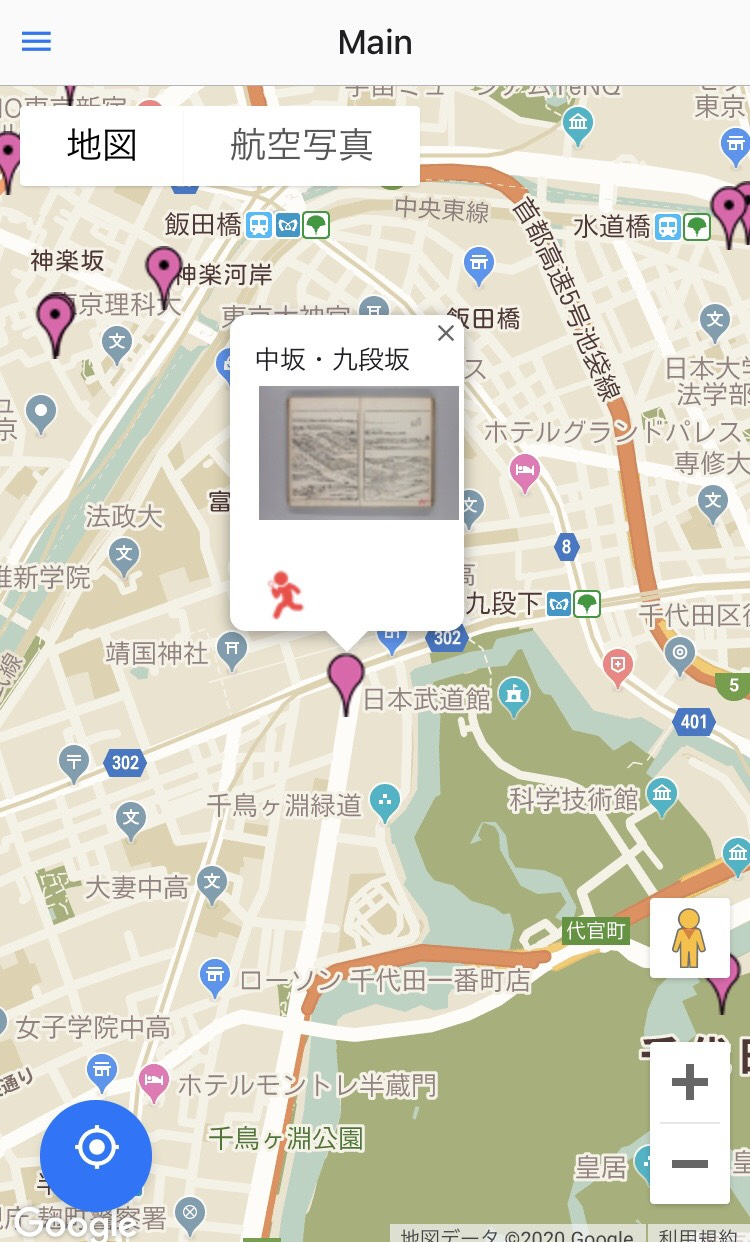
\includegraphics[bb=30 50 550 1300,width=3cm]{./image06.jpg}%%750*1334(100%)でスクショ[大きさ 横 縦,width]
\end{center}
\caption{スタンプ獲得後(黒点なし)}\label{fig:5}
\end{figurehere}

\subsection{ダイアログ表示}
ダイアログを用いて,ピンの詳細情報を表示する機能を実装した(図 6,7 参照).
\begin{figurehere}
\begin{center}
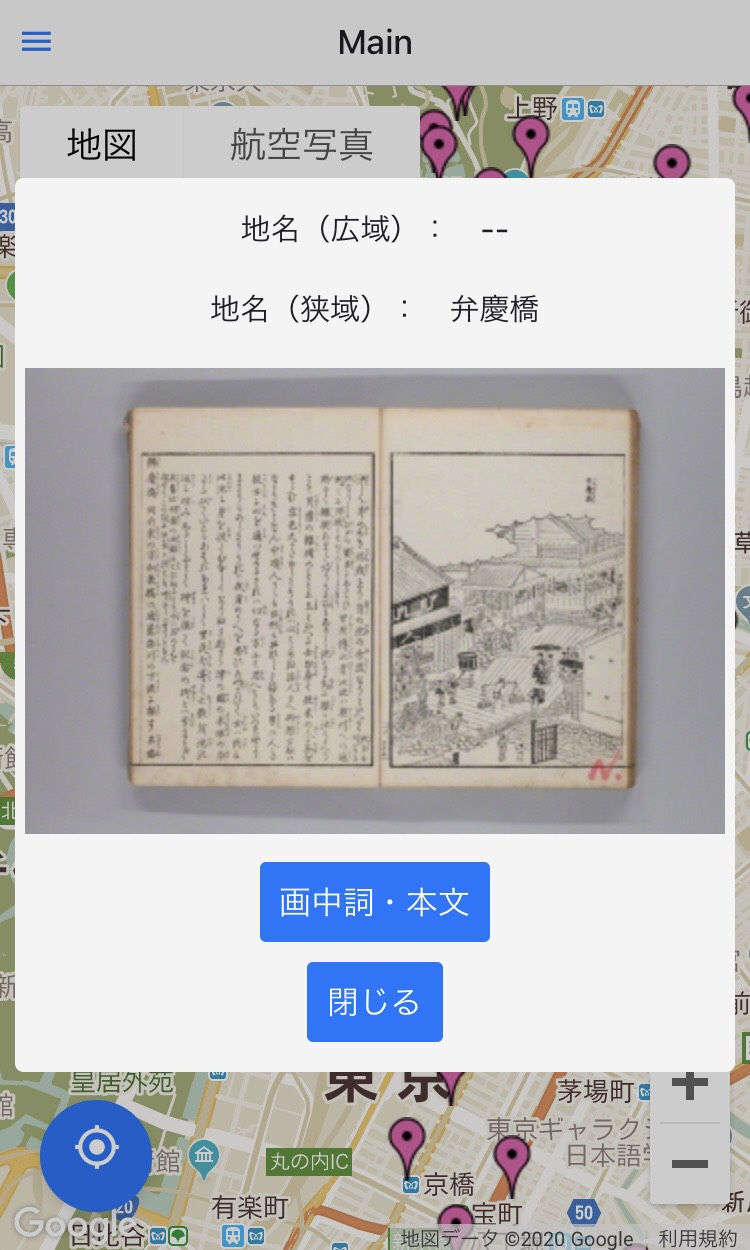
\includegraphics[bb=30 50 550 1300,width=3cm]{./image07.jpg}%%750*1334(100%)でスクショ[大きさ 横 縦,width]
\end{center}
\caption{ダイアログ表示1}\label{fig:6}
\end{figurehere}
\begin{figurehere}
\begin{center}
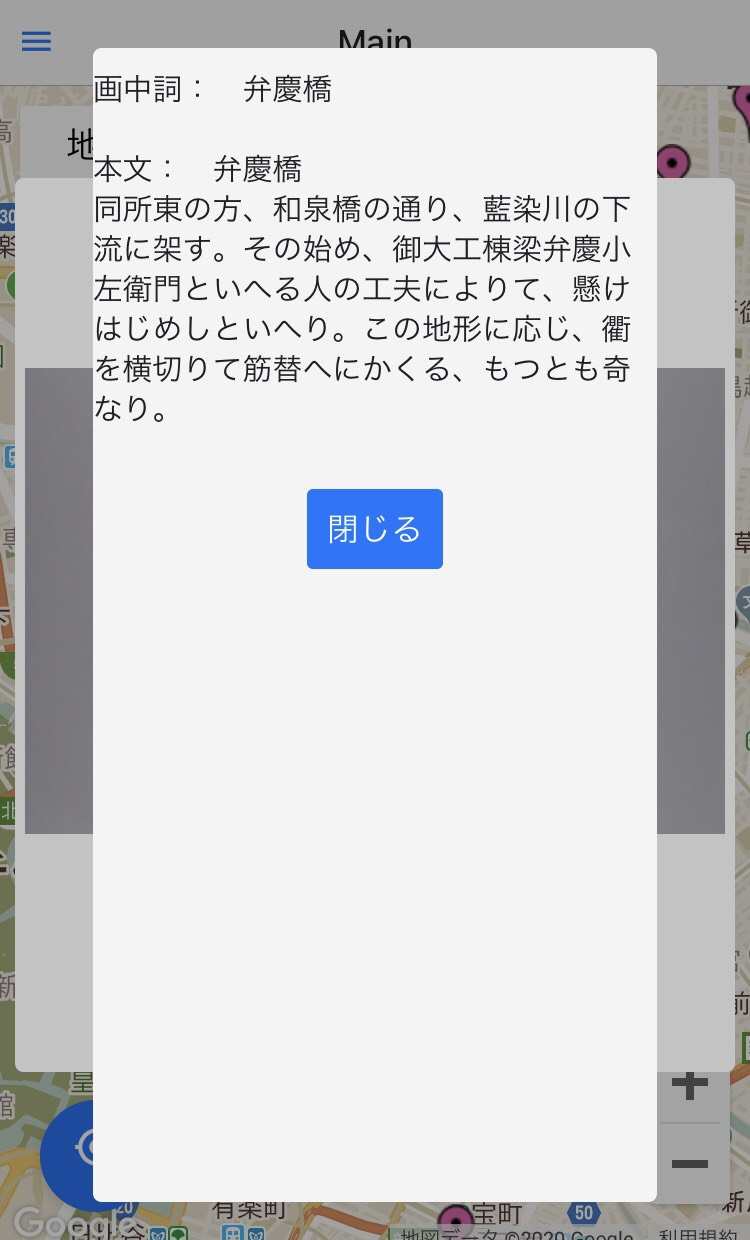
\includegraphics[bb=30 50 550 1300,width=3cm]{./image08.jpg}%%750*1334(100%)でスクショ[大きさ 横 縦,width]
\end{center}
\caption{ダイアログ表示2}\label{fig:7}
\end{figurehere}

\subsection{スプリッター・ステータスバー}
画面左上の三本線のボタンを押すと,画面左からスプリッターが表示される.スプリッターにはピン選択項目があり,表示させたいピンの項目を選択すると,地図上にピンが表示される(図 8,9 参照).
\begin{figurehere}
\begin{center}
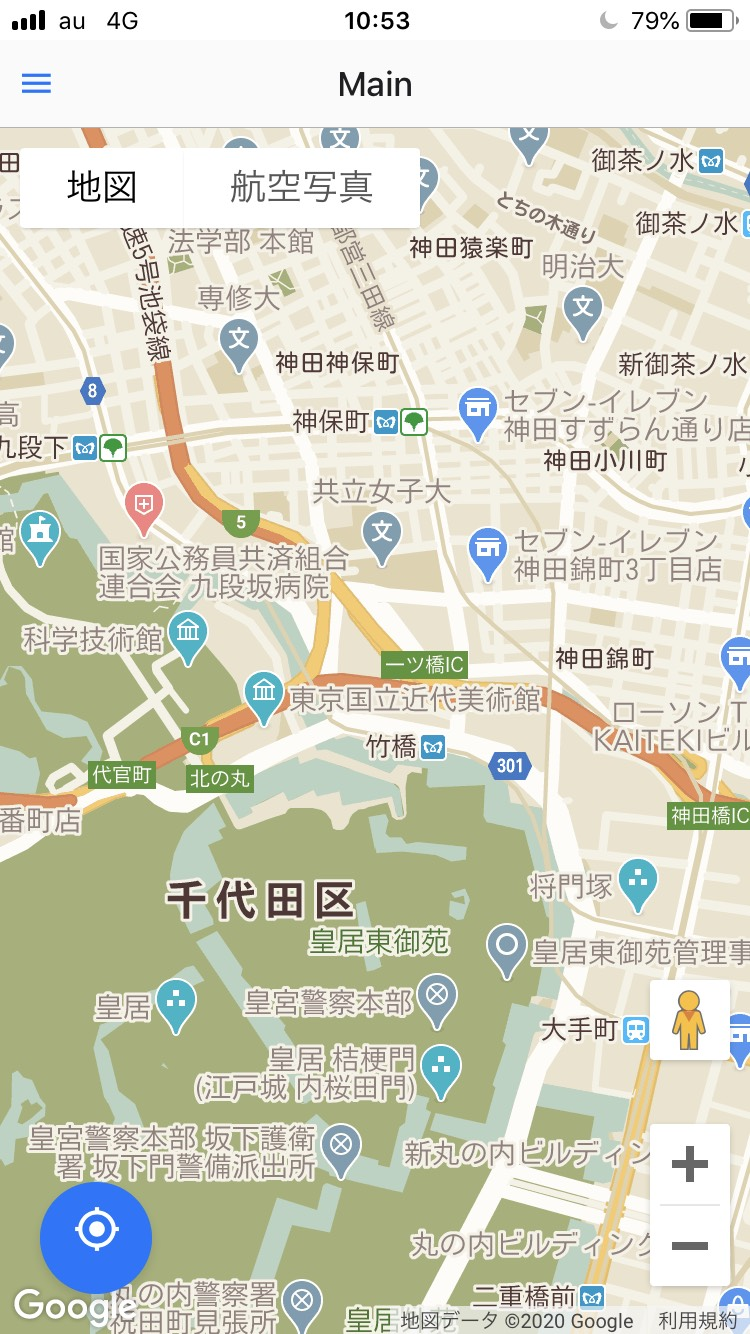
\includegraphics[bb=30 50 550 1300,width=3cm]{./image09-0.jpg}%%750*1334(100%)でスクショ[大きさ 横 縦,width]
\end{center}
\caption{スプリッター・ステータスバー 非表示}\label{fig:8}
\begin{center}
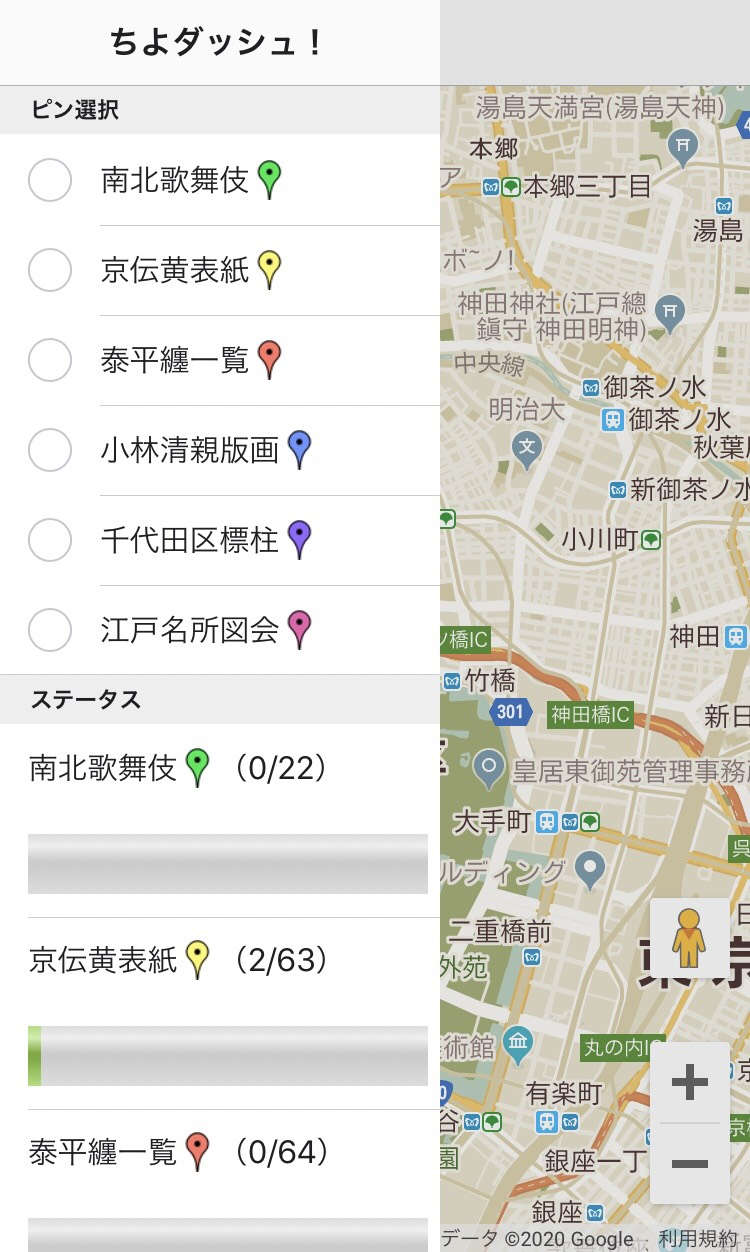
\includegraphics[bb=30 50 550 1300,width=3cm]{./image09.jpg}%%750*1334(100%)でスクショ[大きさ 横 縦,width]
\end{center}
\caption{スプリッター・ステータスバー 表示}\label{fig:9}
\end{figurehere}

また,スプリッターにはステータス項目があり,それぞれのピンの獲得数を棒グラフで確認することができる.さらに,利用規約項目では,いつでも利用規約を確認することができる(図 10 参照).
\begin{figurehere}
\begin{center}
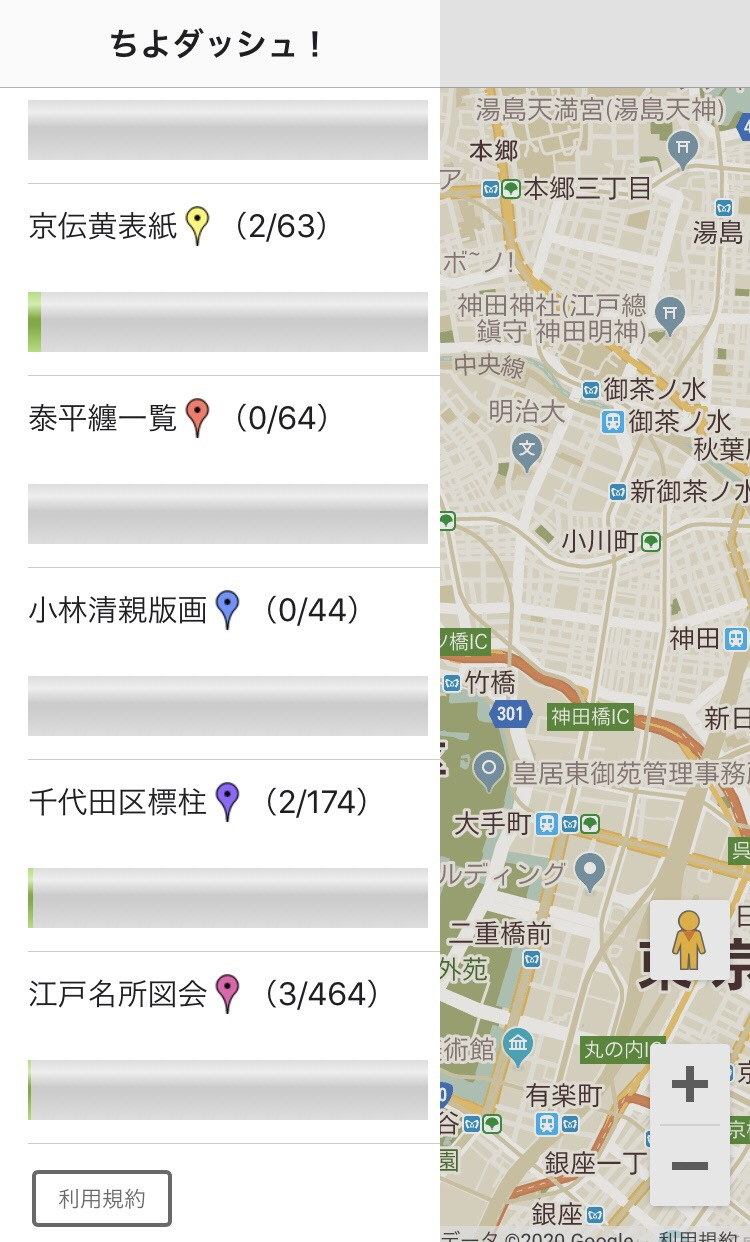
\includegraphics[bb=30 50 550 1300,width=3cm]{./image10.jpg}%%750*1334(100%)でスクショ[大きさ 横 縦,width]
\end{center}
\caption{スプリッター・ステータスバー}\label{fig:10}
\end{figurehere}


\subsection{トースト機能}
ユーザがスタンプを押す時にピンからの距離が遠い場合,またはユーザがアプリに現在地取得を許可しない場合,スタンプを押すことができず画面下から警告としてトーストが表示される(図 11 参照).
\begin{figurehere}
\begin{center}
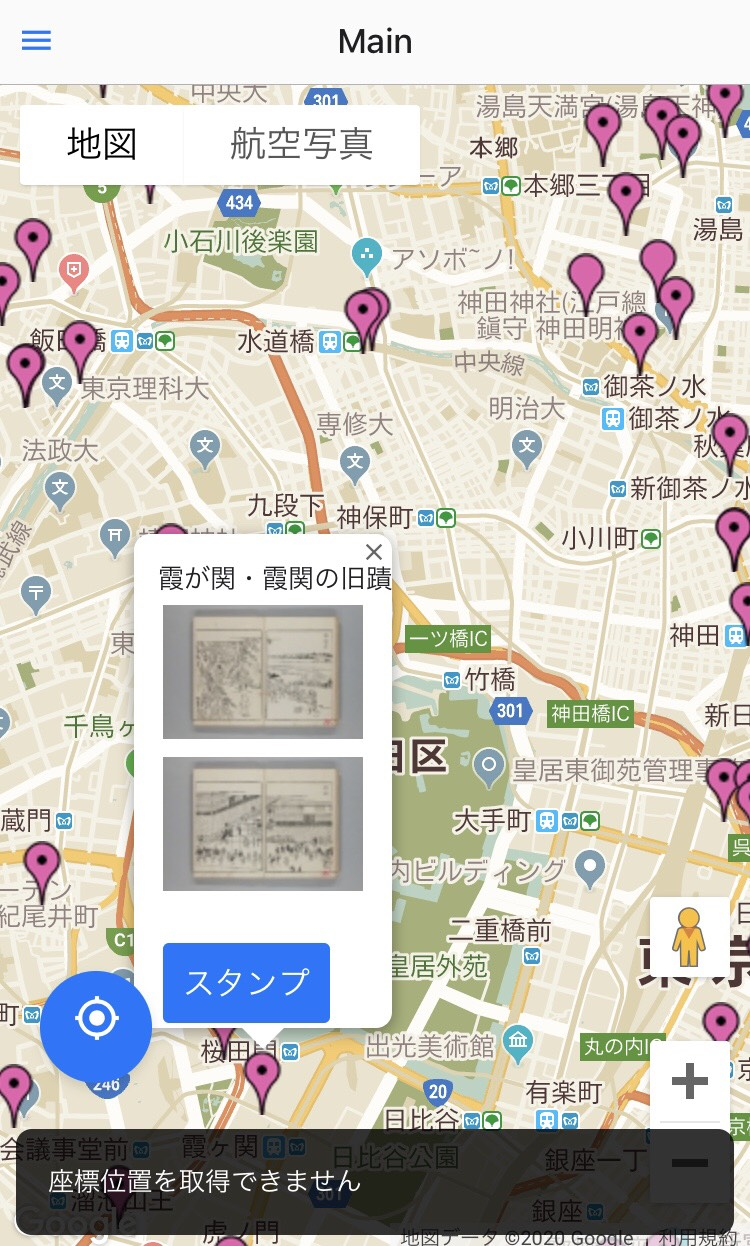
\includegraphics[bb=30 50 550 1300,width=3cm]{./image11.jpg}%%750*1334(100%)でスクショ[大きさ 横 縦,width]
\end{center}
\caption{トースト}\label{fig:11}
\end{figurehere}

% \subsection{現在地自動取得}
% アプリ起動時に自動的に現在地を取得する.また画面左下の青いボタンを押すと任意で現在地を取得することができるようになっている.

% \subsection{ピン表示時のアニメーションの追加}
% ユーザがピンを表示する際にピンが上から落ちてくるようなアニメーションを追加し.

\subsection{仕様}
アプリ起動直後,スプラッシュ画面として「ちよダッシュ!」をイメージした画像が表示され,利用規約画面に遷移する.そして,利用規約に同意すると地図画面に遷移する.
地図画面には Google Maps ,現在位置取得ボタンが表示され,三本線のボタンを押すとスプリッターが表示される.スプリッターには近世,近代,現代の各ジャンルにおける資料のチェックボックスがある.チェックボックスを選択するとその項目に関連した地点にピンが立ち,ピンを選択することで地点に関する資料とスタンプボタンが表示される.スタンプを獲得するには,ユーザがピンの近くに行きスタンプボタンを押す必要がある.現在位置が知りたい場合には,現在地取得ボタンを押すことにより現在位置を取得することができる(図 12 参照).

\begin{figurehere}
\begin{center}
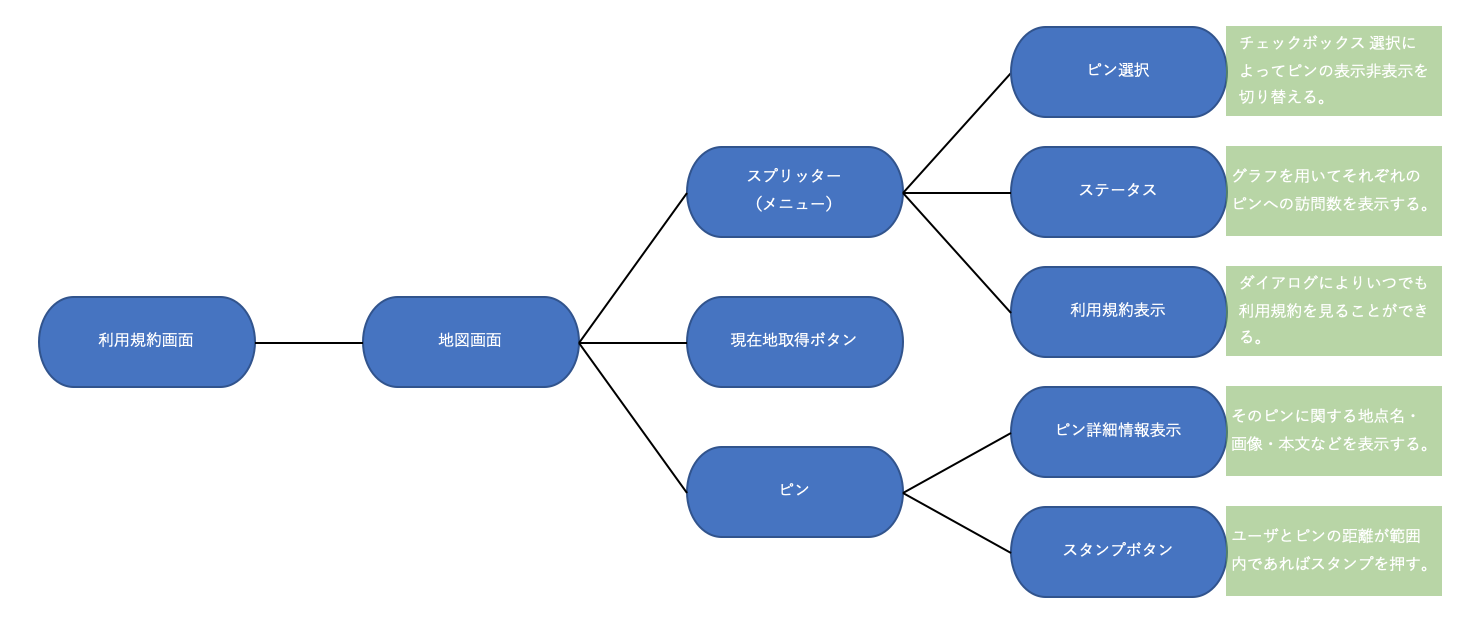
\includegraphics[bb=30 10 700 370,width=7cm]{./image13.png}
%\includegraphics[bb= おおきさ? ]
%%750*1334(100%)でスクショ[大きさ 横 縦,width]
\end{center}
\caption{アプリの遷移図}\label{fig:12}
\end{figurehere}

\subsection{使用した API}
マップとピン情報の表示にあたり「 Google Maps Platform 」を使用した. Google Maps Platform とは, \cite{api}によると「Google社が提供している高機能で世界中の地図データを扱っているGoogleマップを,さまざまなサービスで利用できるようにしたものである. Android や iOS 向けアプリやWebサービスにGoogleマップを使用することができる.」というものである.これを利用することで,マーカー,ライン,色,ポリゴン,画像をカスタマイズして独自の地図を作成することができる.

\subsection{アプリの開発環境}
本演習では Monaca を用いてアプリ開発を行った. Monaca とは, HTML5 , JavaScript などの Web 標準言語でモバイルアプリ開発を行うことができるクラウドベースの開発プラットフォームである.ブラウザ上でコーディングができ, UI のライブプレビューなどの機能を提供している.

\subsection{データベース管理機能}
本演習のデータベース管理は Monaca との連携が容易であるニフクラ mobile backend を利用した.ニフクラ mobile backend とは,文学テキストや言語資料をクラウド上で管理できるクラウドサービスである.会員管理・認証やデータベース管理などの機能も備わっているため,スマートフォンアプリでよく利用される汎用的な機能を導入することができる.

\subsection{ステータスデータ保存方法}
本演習では LocalStorage を用いてステータスデータを端末に保存した. LocalStorage とは, HTML5 から追加された新機能で, JavaScript を利用することでユーザのデータをWebブラウザ(ローカル環境)に保存することができる機能である.

\subsection{アプリとデータ通信に関する関係図}
アプリ起動時にニフクラ mobile backend からピンに関する情報(タイトル・座標・画像データのURL)を取得する.画像データのURLは「江戸・東京WebGIS」のものを利用している.ユーザがスタンプを押すと,その情報はステータス情報として LocalStorage に保存される. LocalStorage に保存することにより,次回起動時にもユーザのステータス情報を引き継いで使うことができる.また,ピン情報はニフクラ mobile backend から取得しているので,アプリのアップデートなしに新規のピンを追加することができる(図 13 参照).
\begin{figurehere}
\begin{center}
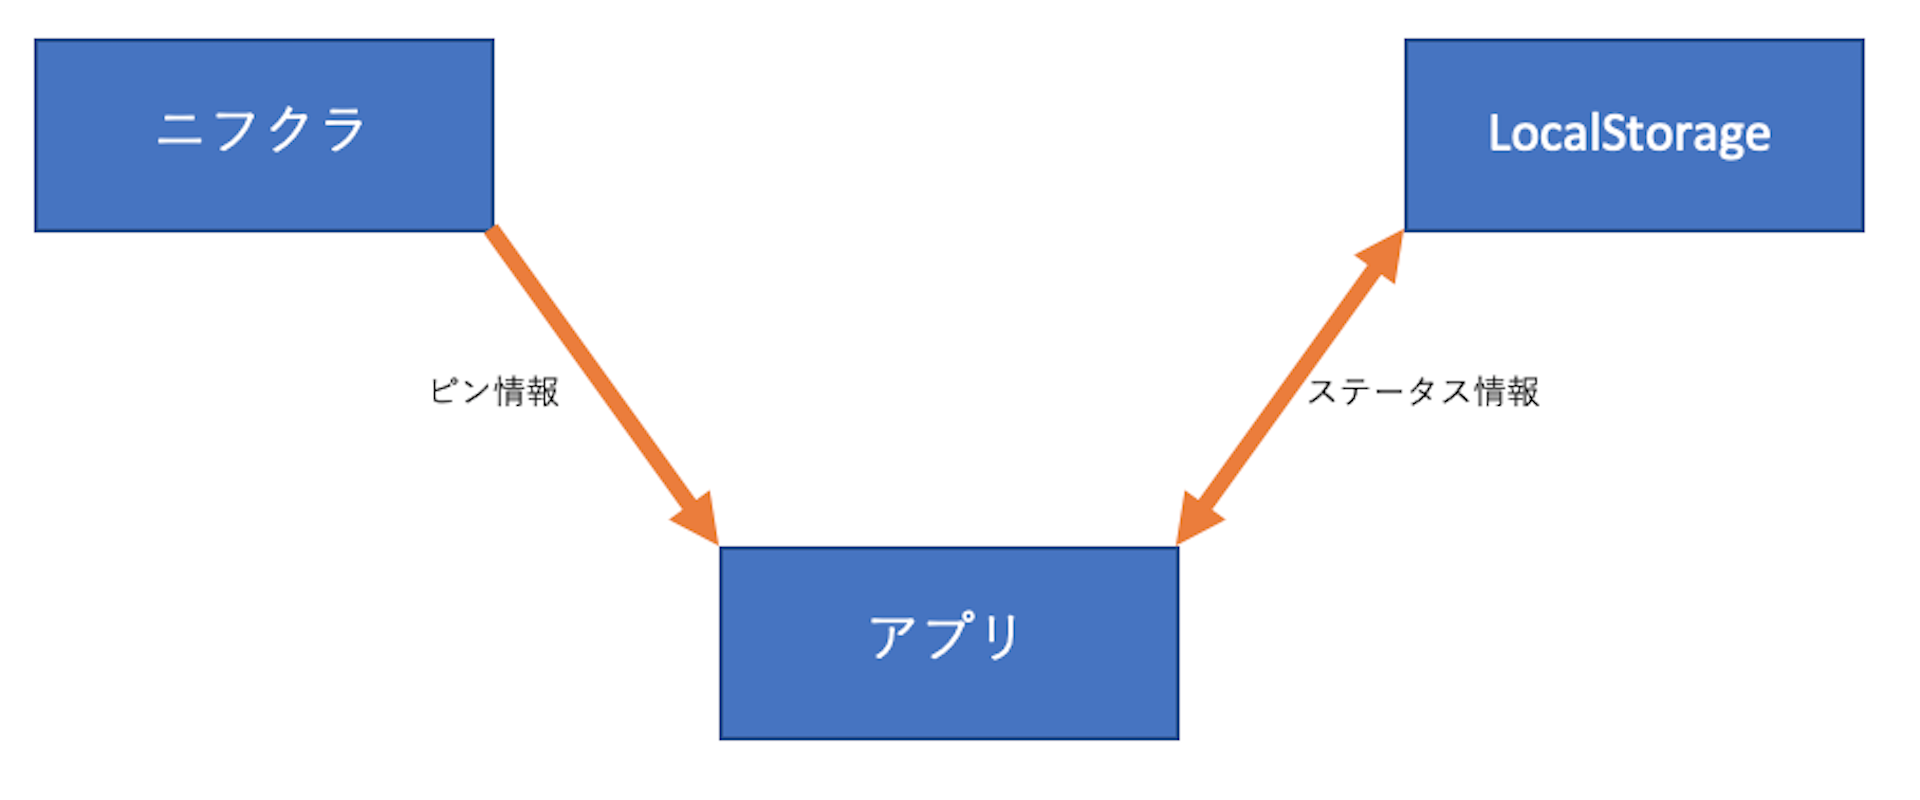
\includegraphics[bb=30 100 550 500,width=3cm]{./image12.png}%%750*1334(100%)でスクショ[大きさ 横 縦,width]
\end{center}
\caption{アプリとデータの関係図}\label{fig:13}
\end{figurehere}


\section{終わりに}
本演習では,昨年度の「ちよダッシュ!」のコンセプトとプロトタイプアプリに基づき,改良・改善を加えた正式版の開発とリリースを行った.開発する上で Monaca ,ニフクラ mobile backend , LocalStorage , Google Maps Platform を使用した.
昨年度の「ちよダッシュ!」にステータス機能を加えることによりゲーム性を高め, GUI を改善することでアプリの利便性を高めた.また,ピンの種類を増やすとともにピン詳細の画像を追加することで,街歩きをより楽しめるようにした.\par
本演習においての課題は,一般公開をすることでユーザから新たに得られた改善点を基に,より使いやすいアプリへ改良することがあげられる.また, Google Maps の更新やニフクラ mobile backend のデータベースの継続的な管理が必要である.



\end{multicols} % 2段落にする(終了)
\vspace{1cm}
% multicols を end したあとに参考文献
\begin{thebibliography}{99}

\bibitem{huma}文部科学省 人文学及び社会科学の意義・役割・目的について\par
http://www.mext.go.jp/b\_menu/shingi/gijyutu/gijyutu4/015/siryo/attach/1343073.htm (参照:2020-03-04)

\bibitem{digihumu1}東京大学大学院横断型教育プログラム デジタル・ヒューマニティーズ\par
http://dh.iii.u-tokyo.ac.jp/ (参照:2020-03-04)
\bibitem{digihumu2}国立情報学研究所(NII) 北本 朝展 デジタル・ヒューマニティーズ\par
http://agora.ex.nii.ac.jp/kitamoto/research/dh/ (参照:2020-03-04)

% \bibitem{h30tiyo}WebGISを用いた千代田ヴァーチャル時空散歩アプリの構築\par
% https://www.city.chiyoda.lg.jp/koho/kurashi/volunteer/documents/nihon30-1gaiyo.pdf (参照:2020-3-04)

% \bibitem{tiyodagaku_houkokusyo} WebGISを用いた千代田ヴァーチャル時空散歩アプリの構築 日本大学・田中ゆかり\par
% https://www.city.chiyoda.lg.jp/koho/kurashi/volunteer/documents/nihon30-1gaiyo.pdf (参照:2020-03-04)

\bibitem{digi4}千代田区役所 区内大学,専修・各種学校等と区の連携協力 平成16年度〜「千代田学」提案制度\par
https://www.city.chiyoda.lg.jp/koho/kurashi/volunteer/renke/index.html (参照:2020-03-04)

% \bibitem{digi5}「千代田学」調査・研究実績報告書\par
% https://www.city.chiyoda.lg.jp/koho/kurashi/volunteer/tean-ichiran.html (参照:2020-2-06)

\bibitem{digi1}千代田区 区の起こり・由来\par
https://www.city.chiyoda.lg.jp/koho/kuse/gaiyo/yokoso/okori.html (参照:2020-03-04)

\bibitem{digi2}日本大学の歴史\par
http://www.nihon-u.ac.jp/history/(参照:2020-03-04)

\bibitem{chiyopro}千代田区内大学と千代田区の連携協力に関する基本協定\par
https://www.city.chiyoda.lg.jp/koho/kurashi/volunteer/renke/kihonkyote.html(参照:2020-03-04)

\bibitem{monka}文部科学省私立大学戦略的研究基盤形成支援事業\par
https://www.mext.go.jp/component/a\_menu/education/detail/\_\_icsFiles/afieldfile/2010/04/23/1267810\_3\_1.pdf (参照:2020-03-04)

% \bibitem{webgis_gaiyo}日本語日本文学半プロジェクト江戸・東京WebGIS概要\par
% http://dep.chs.nihon-u.ac.jp/japanese\_lang/nichigo-nichibun/\#content\_03 (参照:2020-2-06)

\bibitem{houkokusyo_30}平成30年度千代田学研究成果報告書WebGISを用いた千代田ヴァーチャル時空散歩アプリの構築日本大学 田中ゆかり\par
https://www.city.chiyoda.lg.jp/koho/kurashi/volunteer/documents/nihon30-1.pdf (参照:2020-03-04)

\bibitem{tiyokenkyu}「千代田学」調査・研究実績報告書\par
https://www.city.chiyoda.lg.jp/koho/kurashi/volunteer/tean-ichiran.html (参照:2020-03-04)

\bibitem{tiyodagaku_houkokusyo} WebGISを用いた千代田ヴァーチャル時空散歩アプリの構築 日本大学・田中ゆかり\par
https://www.city.chiyoda.lg.jp/koho/kurashi/volunteer/documents/nihon30-1gaiyo.pdf (参照:2020-2-06)

\bibitem{api} 「Google マップを使ってみよう!」\par
https://www.zenrin-datacom.net/business/media/g001/index.html(参照:2020-03-04)

% \bibitem{} (参照:2020-2-06)

% \bibitem{} (参照:2020-2-06)

\end{thebibliography}

\end{document} % 文書(終了)
